\chapter{État de l’art du projet}
{\LARGE \bfseries Introduction\\[0.4cm] }
\noindent\lettrine[lines=2]{\textbf{C}}\\e chapitre se compose de trois parties principales. La première partie présente l’organisme d’accueil, en décrivant ses secteurs d’activité et ses prestations de services. La deuxième partie est dédiée à l’étude de l’existant et à l’analyse critique des solutions disponibles, ce qui nous permet de justifier la solution proposée . Enfin, la troisième partie se concentre sur la méthodologie de travail adoptée pour la réalisation du projet et le formalisme utilisé pour la présentation des résultats.

\section{Présentation de l’organisme d’accueil}
Pour situer notre projet dans son contexte, cette section présente l’organisme d’accueil, ses domaines d’activité ainsi que les services qu’il propose.

\subsection{Groupe Talan}
\textbf{Talan} a été fondé il y a plus de vingt ans par Mehdi Houas, Éric Benamou et Philippe Cassoulat, avec l’objectif de créer un cabinet de conseil centré sur l’innovation et la transformation numérique.
\vspace{0.4cm}\\
Leur ambition était de bâtir un modèle d’entreprise valorisant la diversité des compétences et favorisant le partage équitable de la valeur créée. \vspace{0.4cm}\\
Rapidement, le groupe s’est internationalisé et est aujourd’hui présent sur cinq continents, dans plus de 20 pays, dont la Tunisie, la France, le Canada, le Royaume-Uni, la Suisse, le Luxembourg, la Belgique, l’Espagne et l’Irlande.\\


\subsection{Talan Consulting Tunisie}
La filiale tunisienne de Talan agit comme un centre de développement "nearshore" et regroupe plus de 500 experts spécialisés dans les technologies numériques. L’équipe est composée de professionnels formés dans les principales écoles d’ingénieurs tunisiennes, offrant ainsi une expertise locale solide et adaptée aux besoins des clients internationaux.
\vspace{0.4cm}\\
Les \textbf{services} proposés par \textbf{Talan Tunisie} couvrent plusieurs domaines clés :\\
\begin{itemize}
   

 \item \textbf{ Digital :} Déploiement de centres de services délocalisés, mise en œuvre de projets de transformation digitale, développement web (Java/JEE, .NET, PHP) et mobile (Android/iOS).\\
\item \textbf{Intégration :} Intégration de solutions CRM (Salesforce), ERP (Oracle Forms, EBS), middleware (Tibco) et mise en place de solutions BI et DATA.\\
\item\textbf{ Test : }Coaching et support pour la définition de méthodes de test, exécution de tests manuels, automatisation et utilisation de recettes applicatives tierces.\\
\item \textbf{Support :} Gestion du support applicatif et fonctionnel, suivi des projets, maintenance évolutive et optimisation des activités métiers.\\
\item \textbf{Innovation :} Le centre "Innovation Factory" favorise l’innovation technologique et d’usage en utilisant des technologies comme le Metavers, la Blockchain et l’Intelligence Artificielle.\\
\item \textbf{Cybersécurité :} Conseil en cyber-résilience, confiance digitale, conformité/GRC et Red Teaming.\\
\end{itemize}
Grâce à cette organisation et cette expertise, Talan Tunisie permet à ses clients d’accélérer leurs projets, de réduire leurs coûts et de se libérer des contraintes liées au sourcing et à la gestion des ressources humaines.
\hyperlink{refTalanTunisie}{[1]}\\
La Figure 1.1 présente l’organigramme de Talan Tunisie

\begin{figure}[H]
\begin{center}
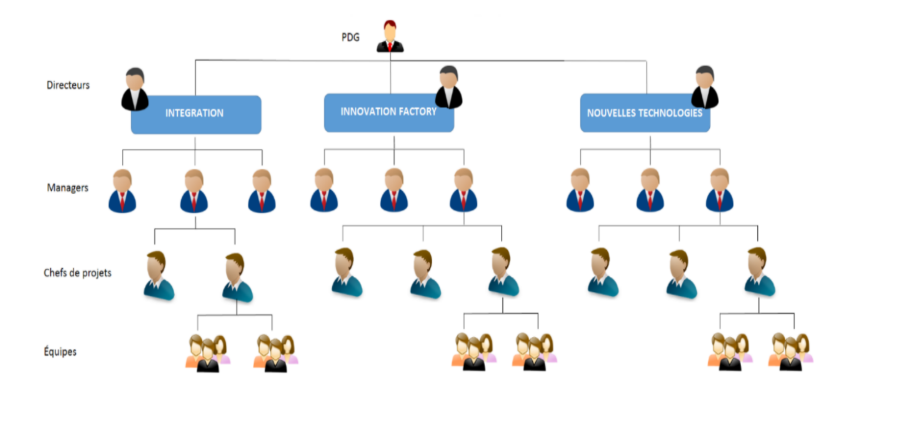
\includegraphics[height=60mm]{images/organigramme_talan_original_cropped.png}
\end{center}
\caption{Organigramme de Talan Tunisie}
\end{figure}


\section{Étude de l’existant}
Pour concevoir Persona Tester, il est essentiel d’analyser les solutions existantes dans le domaine de l’automatisation des tests d’interface et de la simulation utilisateur. Plusieurs outils commerciaux et open source permettent aujourd’hui d’automatiser des tests fonctionnels et visuels, mais chacun présente des limites spécifiques en termes de simulation de comportements réels et d’analytics UX.  



\subsection{Analyse de l'existant}


\subsubsection{Momentic AI}
Momentic AI est une plateforme SaaS spécialisée dans les tests fonctionnels automatisés (UI/regression). Elle fournit une interface no-code intuitive et permet la génération automatique de tests. 
\hyperlink{ref:MomenticAI}{[\ref{ref:MomenticAI}]}  

\begin{itemize}
    \item \textbf{Principales fonctionnalités :}
    \begin{itemize}
        \item Interface no-code intuitive
        \item Génération automatique de tests
        \item Intégration CI/CD native
        \item Maintenance automatique des sélecteurs
    \end{itemize}
    \item \textbf{Limites :}
    \begin{itemize}
        \item Aucun profil comportemental utilisateur
        \item Pas de simulation de personnalité
        \item Pas d'analytics UX
        \item Tarification élevée (Enterprise)
        \item Données hébergées en cloud
    \end{itemize}
\end{itemize}

\subsubsection{Blok AI}
Blok AI est un outil SaaS permettant la validation UX et la détection d'anomalies visuelles. Il est intégré aux design systems et à Figma. 
\hyperlink{ref:BlokAI}{[\ref{ref:BlokAI}]}  

\begin{itemize}
    \item \textbf{Principales fonctionnalités :}
    \begin{itemize}
        \item Détection d'anomalies visuelles
        \item Comparaison avant/après déploiement
        \item Intégration Figma et design system
        \item Rapports visuels
    \end{itemize}
    \item \textbf{Limites :}
    \begin{itemize}
        \item Pas de simulation d'utilisateurs réels
        \item Pas de profils comportementaux
        \item Orienté validation visuelle uniquement
        \item Coût élevé
    \end{itemize}
\end{itemize}

\subsubsection{Browser-Use}
Browser-Use est une bibliothèque open source permettant la navigation web autonome par LLM. Elle est gratuite et facile à intégrer. 
\hyperlink{ref:BrowserUse}{[\ref{ref:BrowserUse}]}  

\begin{itemize}
    \item \textbf{Principales fonctionnalités :}
    \begin{itemize}
        \item Open source et gratuit
        \item Support multi-LLM (GPT, Claude, Ollama)
        \item Boucle ReAct native
        \item Facile à intégrer
        \item Communauté active
    \end{itemize}
    \item \textbf{Limites :}
    \begin{itemize}
        \item Aucune notion de persona comportemental
        \item Pas de métriques UX
        \item Pas d'orchestration multi-agents
        \item Pas de détection de régression
        \item Pas de rapport structuré
    \end{itemize}
\end{itemize}

\subsubsection{ThunderCode}
ThunderCode est une plateforme SaaS combinant génération de tests IA, personas IA autonomes et tests fonctionnels end-to-end. 
\hyperlink{ref:ThunderCode}{[\ref{ref:ThunderCode}]}  

\begin{itemize}
    \item \textbf{Principales fonctionnalités :}
    \begin{itemize}
        \item Génération de test IA à partir du langage naturel
        \item Tests fonctionnels end-to-end
        \item Personas IA autonomes
        \item UI/UX testing
        \item Performance et accessibilité
    \end{itemize}
    \item \textbf{Limites :}
    \begin{itemize}
        \item Outil relativement nouveau sur le marché
        \item Pas de support pour Mobile Testing
        \item Personas principalement techniques, pas de simulation des profils non-techniques
        \item Tarification à partir de 300€/mois pour 1-2 utilisateurs
    \end{itemize}
\end{itemize}

\subsubsection{UXAgent (recherche académique)}
UXAgent est une approche exploratoire visant à améliorer la simulation de comportements utilisateurs dans les tests automatisés. 
\hyperlink{ref:UXAgent}{[\ref{ref:UXAgent}]}  

\begin{itemize}
    \item \textbf{Limites :}
    \begin{itemize}
        \item Encore peu mature pour une intégration industrielle
        \item Manque de support pour tests multi-agent et end-to-end
    \end{itemize}
\end{itemize}

\subsection{Critique de l’existant}
Malgré les avancées significatives des solutions existantes, plusieurs limites persistent. Les plateformes commerciales fournissent des tests automatisés performants, mais elles ne simulent pas de manière réaliste le comportement des utilisateurs et offrent peu d’outils d’analytics UX.\\ Les bibliothèques open source, telles que Browser-Use, apportent flexibilité et personnalisation, mais restent incomplètes pour la génération de rapports structurés et la simulation de personas diversifiés. \\Enfin, certaines approches récentes intègrent des agents autonomes, mais elles sont souvent limitées dans le support mobile et dans la prise en compte des utilisateurs non techniques. Ces lacunes soulignent la nécessité d’une approche plus globale et complète pour l’automatisation et l’analyse comportementale des tests utilisateurs.


\subsection{Solution proposée}

Pour remédier aux limites des solutions existantes et répondre aux besoins identifiés, nous avons conçu une solution intitulée \textbf{Persona Tester}. Cette approche vise à combiner l'automatisation des tests avec la simulation de profils comportementaux variés et l'analyse complète de l'expérience utilisateur.

\subsubsection{Objectifs principaux}
La solution \textbf{Persona Tester} poursuit les objectifs suivants :
\begin{itemize}
    \item Simuler des utilisateurs aux comportements diversifiés pour mieux refléter les usages réels.
    \item Automatiser les tests fonctionnels et d'interface tout en intégrant la dimension UX.
    \item Fournir des métriques détaillées sur la performance, l’accessibilité et la satisfaction utilisateur.
    \item Faciliter l’orchestration de tests sur différentes plateformes (web et mobile) avec une interface intuitive.
\end{itemize}

\subsubsection{Fonctionnalités principales}
La solution intègre plusieurs fonctionnalités clés :
\begin{itemize}
    \item Génération automatique de scénarios de tests à partir de descriptions en langage naturel.
    \item Simulation de personas comportementaux, incluant des profils techniques et non-techniques.
    \item Analyse UX complète, avec visualisation des parcours utilisateurs et reporting structuré.
    \item Intégration continue avec les environnements de développement pour automatiser les tests lors des déploiements.
    \item Support multi-plateforme : web et mobile.
\end{itemize}

\subsubsection{Architecture technique retenue}
L’architecture de \textbf{Persona Tester} repose sur un modèle modulaire :
\begin{itemize}
    \item \textbf{Module de génération} et orchestration des tests, basé sur des agents intelligents.\\
    \item\textbf{ Module de simulation des personas}, capable de reproduire différents comportements utilisateurs.\\
    \item\textbf{ Module d’analyse et reporting}, fournissant des métriques UX et des visualisations détaillées.\\
    \item \textbf{Back-end centralisé }pour la gestion des tests et la collecte des données.\\
    \item\textbf{ Interface front-end} simple et intuitive pour la configuration et la consultation des résultats.
\end{itemize}

\subsubsection{Bénéfices attendus}
La mise en œuvre de \textbf{Persona Tester} devrait permettre :
\begin{itemize}
    \item\textbf{ Une amélioration significative} de la qualité et de la pertinence des tests utilisateurs.\\
    \item \textbf{Une réduction du temps et des coûts} liés à l’exécution manuelle des tests.\\
    \item\textbf{ Une meilleure compréhension} du comportement réel des utilisateurs et de leurs interactions avec l’application.\\
    \item \textbf{Une valorisation de la prise de décision} grâce aux métriques et rapports détaillés fournis.
\end{itemize}

\section{Méthodologie de travail adoptée}

Pour la réalisation de notre projet, nous avons adopté une méthodologie agile basée sur le cadre Scrum. Cette approche permet de structurer le travail en itérations courtes et régulières, de mieux collaborer en équipe et de s’adapter rapidement aux changements et aux imprévus. L’utilisation de Scrum assure également une amélioration continue grâce aux mécanismes de feedback et de rétrospective, garantissant la qualité et la pertinence de la solution développée. \hyperlink{ref:AgileScrum}{[\ref{ref:AgileScrum}]}\\

La figure 1.2 illustre la méthodologie Scrum adoptée pour la gestion et l’organisation du projet.
\begin{figure}[H]
\begin{center}
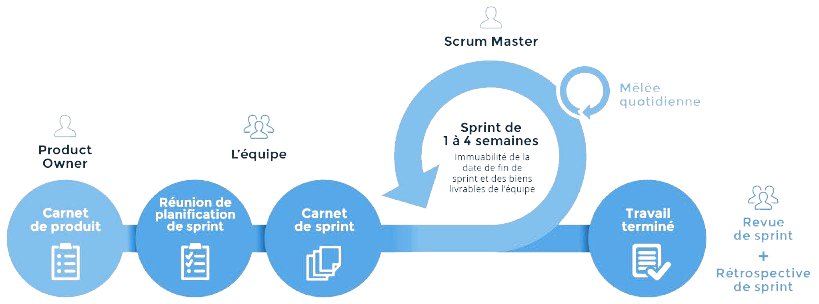
\includegraphics[height=60mm]{images/AgileSCRUM-removebg-preview.png}
\end{center}
\caption{Méthodologie Scrum}
\end{figure}


\subsection{Éléments de Scrum}

Scrum repose sur plusieurs éléments fondamentaux permettant d’organiser et de suivre le projet :
\begin{itemize}
    \item \textbf{Sprint} : période fixe (généralement 2 à 4 semaines) durant laquelle l’équipe développe un ensemble de fonctionnalités.\\
    \item \textbf{Product Backlog} : liste priorisée de toutes les fonctionnalités et exigences du projet, gérée par le Product Owner.\\
    \item \textbf{Sprint Backlog} : ensemble des tâches sélectionnées pour un sprint particulier, détaillant le travail à accomplir. C’est une partie du Product Backlog que l’équipe s’engage à réaliser pendant le sprint.\\
    \item \textbf{Sprint Backlog} : ensemble des tâches sélectionnées pour un sprint particulier, détaillant le travail à accomplir.\\
    \item \textbf{Daily Scrum} : réunion quotidienne de courte durée permettant à l’équipe de synchroniser ses actions et identifier les obstacles.\\
    \item \textbf{Rétrospective} : réunion à la fin de chaque sprint pour analyser ce qui a bien fonctionné, ce qui peut être amélioré et définir des actions correctives.
\end{itemize}

\subsection{Rôles dans l’équipe Scrum}

La réussite de Scrum repose sur une répartition claire des rôles :\\
\begin{itemize}
    \item \textbf{Product Owner} : responsable de la définition des besoins, de la priorisation du Product Backlog et de la validation des livrables.\\
    \item \textbf{Scrum Master} : facilite le processus Scrum, aide l’équipe à lever les obstacles et veille à l’application des bonnes pratiques.\\
    \item \textbf{Équipe de développement} : composée de développeurs, designers et testeurs qui réalisent le travail technique et livrent les fonctionnalités.
\end{itemize}

\subsubsection{Mécanisme de feedback}

Le feedback constitue un levier essentiel pour garantir la qualité du produit final et assurer son adéquation avec les besoins métier. Tout au long du projet, le stagiaire bénéficie de retours réguliers grâce à plusieurs pratiques mises en place dans le cadre de la méthodologie Scrum :\\

\begin{itemize}
    \item \textbf{Les réunions quotidiennes (Daily Scrum)} : elles permettent de suivre l’avancement des tâches, d’identifier les éventuels obstacles et d’obtenir un feedback rapide, notamment en présence du Product Owner.\\
    
    \item \textbf{Les réunions de Sprint Review} : organisées à la fin de chaque sprint, elles consistent à présenter les fonctionnalités développées aux parties prenantes afin de recueillir leurs retours et suggestions.\\
    
    \item \textbf{Les échanges continus avec le Product Owner et le Scrum Master} : ces interactions fréquentes assurent une meilleure compréhension des besoins et permettent d’ajuster le développement en fonction des attentes du client.
\end{itemize}

Ces mécanismes de feedback favorisent une amélioration continue du produit et garantissent un alignement permanent entre les fonctionnalités développées et les objectifs du projet.



\subsection{Chronogramme du projet}


\section{Conclusion}
Ce chapitre a présenté le contexte général du projet, en introduisant l’organisme d’accueil ainsi que ses domaines d’activité. Il a également permis d’analyser les solutions existantes dans le domaine, en mettant en évidence leurs fonctionnalités et leurs limites. Cette étude a conduit à la proposition d’une solution adaptée répondant aux besoins identifiés. Enfin, la méthodologie de travail adoptée, basée sur Scrum, a été décrite afin d’encadrer la réalisation du projet de manière structurée et efficace.

